\documentclass{beamer}
% imprimir
% \documentclass[handout]{beamer} 
% \usepackage{pgfpages}
% \pgfpagesuselayout{4 on 1}[a4paper,landscape,border shrink=5mm]

\mode<presentation> {
  \usetheme{Warsaw}
  \setbeamercovered{transparent}
}

\usebackgroundtemplate{
\includegraphics[width=\paperwidth]{format/libresoft-bg.png}}
\usepackage[spanish]{babel}
\usepackage[utf8]{inputenc}
\usepackage{graphics}
\usepackage{hyperref}
\usepackage{amssymb} % Simbolos matematicos

%\definecolor{libresoftgreen}{RGB}{162,190,43}
%\definecolor{libresoftblue}{RGB}{0,98,143}

%\setbeamercolor{titlelike}{bg=libresoftgreen}

%% Metadatos del PDF.
\hypersetup{  
  pdftitle={Clusters de Alta Disponibilidad},
  pdfauthor={Miguel Vidal},
  pdfcreator={GSyC/Libresoft},
  pdfproducer=PDFLaTeX,
  pdfsubject={Master on Free Software},
}
%%

\begin{document}

\title{Clusters de Alta Disponibilidad}
\subtitle{Master on Free Software}
\institute{\{mvidal,jfcastro\}@libresoft.es} 
\author{Miguel Vidal, José Castro}
%\date{\today}
\date{15 de abril de 2011}

\frame{
\maketitle
\begin{center}

\includegraphics[width=6cm]{format/gsyc-urjc}
\end{center}
}

%% License slide
\begin{frame}
  \vspace{2cm}
  \begin{flushright}
    {\footnotesize \copyright{} 2011 Miguel Vidal, Jose Castro.} \\
%    \vspace{0.25cm}
    \medskip
    {\scriptsize Esta presentación se distribuye bajo \\ licencia Creative Commons Reconocimiento 3.0 España}
%    \vspace{0.10cm}
  \end{flushright}
  \begin{center}
    \href{http://creativecommons.org/licenses/by/3.0/es}{
\includegraphics[width=2cm]{format/cc-by.png}} \\
    {\tiny \url{http://creativecommons.org/licenses/by/3.0/es}}
  \end{center}
\end{frame}%%


\normalsize


%%%%%%%%%%%%%%%%%%%%%%%%%%%%%%%%%%%%%%%%%%%%%%%%%%%%%%%%%%%%%%%%%%%%%%%

\begin{frame}
\frametitle{¿Qué es un clúster HA?}


\begin{itemize}
\item \alert{Conjunto de máquinas unidas por red} (clúster), orientado a ofrecer y garantizar servicios en \alert{Alta Disponibilidad} (24/7, con alto grado de fiabilidad y de continuidad operativa).
\item Se basa en 2 o más máquinas redundantes (\textit{nodos}), que asumen el servicio cuando algún componente del sistema falla.

	\begin{itemize}
	\item \alert{Nodos maestros}: donde normalmente se ejecuta el servicio.
	\item \alert{nodos esclavos}, \alert{backups} o \alert{pasivos}: despliegan los servicios en el caso de que el nodo maestro falle. 
	\end{itemize}

\item Su propósito es eliminar los \alert{Puntos Únicos de Fallo} (SPoF), mediante redundancia a todos los niveles, desde el hardware hasta el almacenamiento o las conexiones de red. 

\end{itemize}

\end{frame}

%%%%%%%%%%%%%%%%%%%%%%%%%%%%%%%%%%%%%%%%%%%%%%%%%%%%%%%%%%%%%%%%%%%%%%%

\begin{frame}
\frametitle{Misión de un clúster HA}

Un clúster HA debe ser capaz de: 

\begin{itemize}
\item detectar cualquier fallo de hardware o de software (desde denegación de servicio o bloqueo del sistema operativo hasta problemas a nivel de aplicación)
\item reiniciar la aplicación en otro nodo
\item mantener el servicio sin intervención de operador alguno
\item garantizar la integridad de los datos del clúster
\end{itemize}

Este proceso (\alert{failover}) incluye otras operaciones previas automatizadas, como montar el sistema de ficheros, asignarse la IP, etc. 

\end{frame}

%%%%%%%%%%%%%%%%%%%%%%%%%%%%%%%%%%%%%%%%%%%%%%%%%%%%%%%%%%%%%%%%%%%%%%%

\begin{frame}
\frametitle{Tipos de configuración}

\begin{itemize}
\item El tamaño más frecuente de un clúster HA es de \alert{2} nodos (mínimo requerido).
\item Los dos configuraciones más comunes en los clusters de dos nodos son \alert{activo/pasivo} y \alert{activo/activo}.
	\begin{itemize}
	\item \alert{Clúster activo/pasivo}: hay un solo nodo dando servicio.
	\item \alert{Clúster activo/activo}: todos los nodos se encuentran dando servicio.
	\end{itemize}
\item \alert{N+1}: Un nodo extra que puede asumir las funciones de cualquiera de los nodos que haya fallado.

\end{itemize}

\end{frame}


%%%%%%%%%%%%%%%%%%%%%%%%%%%%%%%%%%%%%%%%%%%%%%%%%%%%%%%%%%%%%%%%%%%%%%%

\begin{frame}
% \frametitle{Clúster HA de 2 nodos}

\begin{figure}[h]

\begin{center}
  \centering
  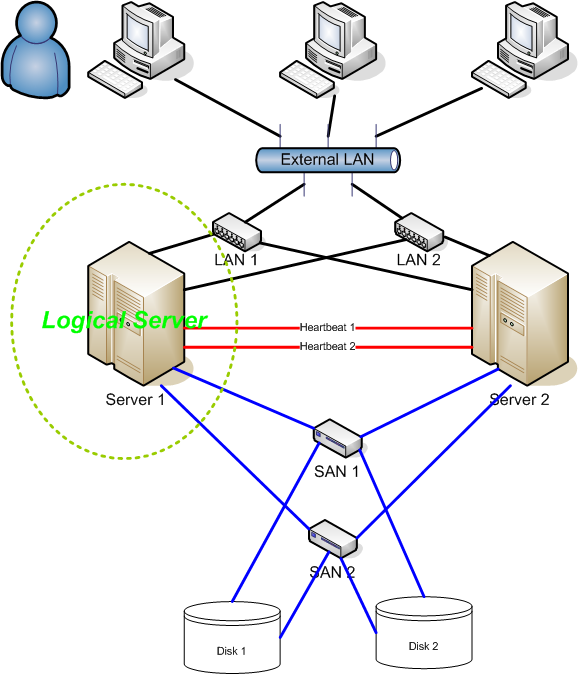
\includegraphics[height=2.7in]{figs/2nodeHAcluster.png}
  \caption{Clúster HA de 2 nodos. \textit{Fuente:} Wikipedia.}
\end{center}
\end{figure}

\end{frame}


%%%%%%%%%%%%%%%%%%%%%%%%%%%%%%%%%%%%%%%%%%%%%%%%%%%%%%%%%%%%%%%%%%%%%%%

\begin{frame}
\frametitle{Conceptos básicos}

\begin{itemize}
\item \alert{Failover}: recuperación de un fallo desplegando los servicios en otro nodo.
\item \alert{Heartbeat}: pulso o ``latido'' mediante el cual se mantiene la comunicación entre los nodos del clúster. 
\item \alert{Split-brain}: cuando los enlaces de red que unen a los nodos entre sí caen, pero los nodos siguen operando. 
\item \alert{Stonith} (``Shoot The Other Node In The Head''): una de las técnicas de \alert{fencing} (bloqueo de recursos en estado incierto). Ambos nodos se ``apuntan'' uno al otro: al detectar que un nodo está caído, el otro nodo le enviará un comando ``reset''. También se usa como técnica de recuperación automática para desbloquear un nodo.
\item \alert{Agente de recurso}: un interfaz estándar para manejar los recursos del cluster (red, montaje de filesystems, servicios, etc.). 
\end{itemize}

\end{frame}

%%%%%%%%%%%%%%%%%%%%%%%%%%%%%%%%%%%%%%%%%%%%%%%%%%%%%%%%%%%%%%%%%%%%%%%

\begin{frame}
\frametitle{Referencias}

\begin{itemize}
\item Linux HA Project: \href{http://www.linux-ha.org}{http://www.linux-ha.org}
\item \textsc{Miguel Vidal, José Castro}: \href{http://www.ati.es/novatica/2011/209/Nv209-75.pdf}{``Creación de un clúster de Alta Disponibilidad''}, \textit{Novática}, nº 209, marzo de 2011. 
\end{itemize}

\end{frame}




%%%%%%%%%%%%%%%%%%%%%%%%%%%%%%%%%%%%%%%%%%%%%%%%%%%%%%%%%%%%%%%%%%%%%%


\frame{
\maketitle
\begin{center}

\includegraphics[width=6cm]{format/gsyc-urjc}
\end{center}
}



\end{document}




